% chapter 3 section 3

\section{光波}

光作为波的基本信息与第一节的内容相同,故在此略过,仅区分两个用语\footnote{为避免混淆,统一使用日语}。
\begin{itemize}
    \item 分散:虹、スペクトル(折射率不同导致)
    \item 散乱:青空、チンダル現象
\end{itemize}
其中分散现象由于折射率不同导致,体现光的波动性。而散乱现象主要体现光的粒子性,通俗地讲就是一些“跑偏”的光。

\subsection{光的折射}
\label{subsec:3.3.1}

\subsubsection{平行层}

由于$\sin\theta_in_i=const$,所以无论中间途径多少层不同的介质,最终的出射光线都会与入射光线平行。
\begin{figure}[ht!]
    \centering
    \begin{tikzpicture}
        \filldraw[color=black, fill=gray, fill opacity=0.3] (0,0) rectangle (4,0.5);
        \filldraw[color=black, fill=gray, fill opacity=0.8] (0,0.5) rectangle (4,1);
        \draw[thick, midarrow] (0.5,2) -- (1,1);
        \draw[thick, midarrow] (1,1) -- (2.3,0.5);
        \draw[thick, midarrow] (2.3,0.5) -- (3,0);
        \draw[thick, midarrow] (3,0) -- (3.5,-1);
    \end{tikzpicture}
    \caption{平行层折射}
\end{figure}

\subsubsection{水中视差}

从空气中观察水中物体,由于光的折射,实物总会比看起来的更深。其中实际深度$h$和视觉深度$h^\prime$满足$\frac{h}{n}=h^\prime$的关系。
\begin{figure}[ht!]
    \centering
    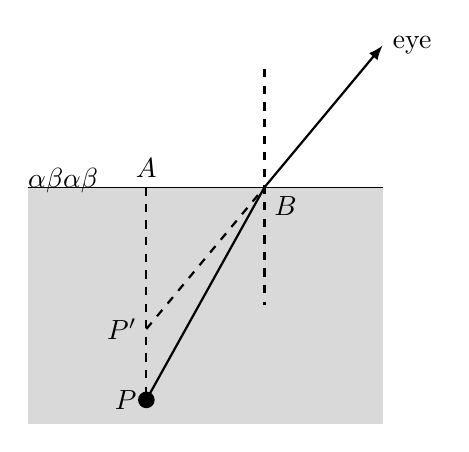
\begin{tikzpicture}[scale=1.5]
        \fill[fill=gray, opacity=0.3] (0,0) rectangle (3,-2);
        \draw (0,0) -- (3,0);
        
        \coordinate (A) at (1,0); \node[above] at (A) {$A$};
        \coordinate (B) at (2,0); \node[below right] at (B) {$B$};
        \coordinate (P) at (1,-1.8); \node[left] at (P) {$P$};
        \coordinate (PP) at (1,-1.2); \node[left] at (PP) {$P^\prime$};
        
        \fill (P) circle (2pt);

        \draw[thick, -latex] (P) -- (B) -- (3,1.2) node[right] {eye};
        \draw[thick, dashed] (PP) -- (B);
        \draw[thick, dashed] (A) -- (P);
        \draw[thick, dashed] (2,1) -- (2,-1);
        \drawangle[$\alpha$]{(B)}{(PP)}{(A)};
        \drawangle[$\beta$]{(B)}{(P)}{(A)};
        \drawangle[$\alpha$]{(3,1.2)}{(B)}{(2,1)};
        \drawangle[$\beta$]{(P)}{(B)}{(2,-1)};
    \end{tikzpicture}
    \caption{水中视差}
\end{figure}
\begin{equation*}
    AB=h^\prime\tan\alpha=h\tan\beta
    \xrightarrow[\tan\approx\sin]{\sin\alpha=\sin\beta n}
    h^\prime=\frac{h}{n}
\end{equation*}

\subsubsection{透镜}

当给定透镜的部分定量信息后,通过透镜公式便可以其他相关定量信息。
\begin{itembox}[l]{透镜公式}
    \begin{equation*}
        \frac{1}{a}+\frac{1}{b}=\frac{1}{f}
    \end{equation*}
    \begin{itemize}
        \item 参数:
        \begin{center}
            \renewcommand\arraystretch{1.2}
            \begin{tabular}{c|cc}
                \hline
                参数&正数&负数\\\hline
                焦距f&凸透镜&凹透镜\\
                物距a&实物&虚物\\
                相距b&实相&虚像\\\hline
            \end{tabular}
        \end{center}
        \item 倍率:$m=\left\lvert\frac{b}{a}\right\rvert$
    \end{itemize}
\end{itembox}

\subsection{光的干涉}
l\label{subsec:3.3.2}

\subsubsection{双缝干涉}

\paragraph{实验内容}双缝实验是英国科学家托马斯杨于1807年为了验证光的波动性所做的实验。从光源$S_0$发出的单色光,通过双缝$S_1$和$S_2$投射到光屏上,其中相比于双缝的间距$d$,光屏的距离$l$足够远。实验发现光屏上会呈现出明暗相间的条纹。
\begin{figure}[ht!]
    \centering
    \begin{tikzpicture}[scale=1.5]
        \draw[thick] (-0.5,0.3) -- (-0.5,-0.3);
        \draw[thick] (0,1) -- (0,0.55);
        \draw[thick] (0,0.45) -- (0,-0.45);
        \draw[thick] (0,-0.55) -- (0,-1);
        \draw (0,0) -- (3.5,0);
        \draw (3,-1) -- (3,1) -- (3.5,1);
        \draw[<->] (3.4,0) -- node[fill=white] {$x$} (3.4,1);

        \coordinate (S0) at (-0.5,0); \node[left] at (S0) {$S_0$};
        \coordinate (S1) at (0,0.5); \node[above left] at (S1) {$S_1$};
        \coordinate (S2) at (0,-0.5); \node[below left] at (S2) {$S_2$};
        \coordinate (H) at (0.4,-0.3); \node[below] at (H) {$H$};
        \coordinate (P) at (3,1); \node[above] at (P) {$P$};

        \draw[dashed] (S1) -- (-1.5,0.5);
        \draw[dashed] (S2) -- (-1.5,-0.5);
        \draw[<->] (-1.4,0.5) -- node[fill=white] {$d$} (-1.4,-0.5);
        \draw[<->] (0,-0.8) -- node[fill=white] {$l$} (3,-0.8);
        \draw[midarrow] (S0) -- (S1) -- (P);
        \draw[midarrow] (S0) -- (S2) -- (P);
        \draw[dashed] (0,0) -- (P);
        \draw[dashed] (0,0.5) -- (H);
        \drawangle[]{(S2)}{(S1)}{(H)};
        \drawangle{(3,0)}{(0,0)}{(P)};
    \end{tikzpicture}
    \caption{双缝干涉}
\end{figure}

\paragraph{干涉条件}根据图形关系可知,两束光线到达$P$点距离的差值为$|S_1P-S_2P|=\frac{dx}{l}$,再结合平面波干涉的结论可得双缝干涉条件。
\begin{itembox}[l]{双缝干涉条件}
    \begin{equation*}
        \frac{dx}{l}=
        \begin{cases}
            2m\cdot\frac{\lambda}{2}&\implies\textrm{明线}\\
            (2m+1)\cdot\frac{\lambda}{2}&\implies\textrm{暗线}
        \end{cases}
    \end{equation*}
\end{itembox}

\paragraph{条纹间距}基于相邻两次干涉位置可求双缝干涉的条纹间距。
\begin{equation*}
    \Delta x=x_m-x_{m-1}=\frac{l\lambda}{d}
\end{equation*}
因此,若是知道$l$,$d$,$\Delta x$的信息即可反向求出波长。

\paragraph{颜色变化}另外,如果光源发出的是全色光则会发现$x=0$的位置出现白色条纹,其两侧由紫色向红色渐变展开。因为对于所有颜色的光$x=0$的位置永远是第零次加强的位置,所以全部汇聚于此,呈现白色。再根据条纹间距可知,波长较短的紫色会离其第零次干涉位置更近,所以白色旁边先会出现紫色。

\paragraph{回折格子}即布满等距缝隙的薄片,其实验原理与双缝干涉一致,只是同时相互干涉的光线更多。因此,不同于双缝干涉,回折格子的明线会更加明显。在此只给出结论。
\begin{itembox}[l]{回折格子干涉条件}
    \begin{equation*}
        d\sin\theta=m\lambda
    \end{equation*}
\end{itembox}

\subsubsection{薄膜干涉}

\paragraph{反射相变}光波在发生反射时根据接触面光学性质的不同会发生位相的变化。在此将折射率大的介质称为\underline{光密},相反称折射率小的介质称为\underline{光疏}。
\begin{figure}[ht!]
    \centering
    \renewcommand\arraystretch{1.2}
    \begin{tabular}{c|cc}
        \hline
        反射&反射端&相变\\\hline
        光密$\to$光疏&自由端&0相变\\
        光疏$\to$光密&固定端&$\pi$相变\\\hline
    \end{tabular}
    \caption{反射相变}
\end{figure}

\paragraph{光程}日文为光学距離,指在统一相位变化的前提下描述光波走行距离的量,并且简称光程相等的两条路径\underline{等光程}。我们在所有干涉实验中着眼的便是这个物理量。
\begin{figure}[ht!]
    \centering
    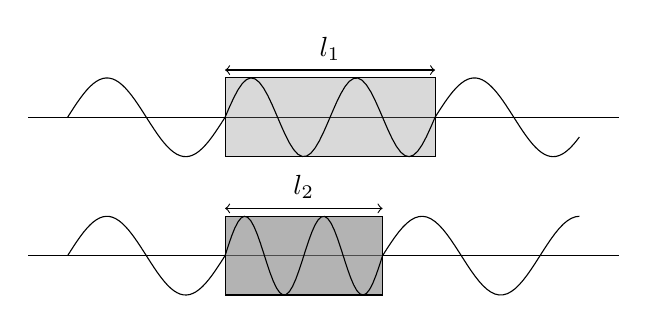
\begin{tikzpicture}
        \foreach \n [count=\i] in {1.5, 2} {
            \begin{scope}[yscale=0.5, yshift={-100*(\i-1)}]
                \draw (-2.5,0) -- (5,0);
                \filldraw[color=black, fill=gray, fill opacity={0.3*\i}] (0,-1) rectangle ({4/\n},1);
                \draw[domain=-2:0] plot[samples=50] (\x, {sin((pi*\x) r)});
                \draw[domain=0:{4/\n}] plot[samples=50] (\x, {sin((\n*pi*\x) r)});
                \draw[domain={4/\n}:4.5] plot[samples=50] (\x, {sin((pi*(\x-4/\n)) r)});
                \draw[<->] (0,1.2) -- node[above] {$l_\i$} ({4/\n},1.2);
            \end{scope}
        }
    \end{tikzpicture}
    \caption{光程}
\end{figure}
\begin{itembox}[l]{光程公式}
    \begin{equation*}
        L=nl
    \end{equation*}
\end{itembox}

\paragraph{实验内容}空间中有一层薄膜,光波斜向而来,观察在膜的表面与底层发生反射的两束光线。实验发现,在膜的表面会出现明暗相间的干涉条纹。
\begin{figure}[ht!]
    \centering
    \begin{tikzpicture}[scale=0.8]
        \fill[fill=gray, opacity=0.3] (0,0) rectangle (6,-2);
        \draw (0,0) -- (6,0);
        \draw (0,-2) -- (6,-2);

        \draw[thick, midarrow] (1,1) -- (2,0);
        \draw[thick, midarrow] (2,2) -- (4,0);
        \draw[thick, -latex] (4,0) -- (5,1);
        \draw[thick] (2,0) -- (3,-2) -- (4,0);

        \node[below left] at (2,0) {$A$};
        \node[below right] at (4,0) {$B$};
        \node[below left] at (3,-2) {$C$};
        \node[right] at (4,-4) {$C^\prime$};
        \node[above right] at (3,1) {$D$};
        \node[right] at (2.4,-0.8) {$H$};

        \draw[dashed] (2,-1) -- (2,1);
        \draw[dashed] (2,0) -- (3,1);
        \draw[dashed] (2.4,-0.8) -- (4,0) -- (4,-4) -- (3,-2);
        \draw[dashed, <->] (0.1,0) -- node[right] {$d$} (0.1,-2);

        \drawangle[$\theta$]{(2,1)}{(2,0)}{(1,1)};
        \drawangle[$\phi$]{(2,-1)}{(2,0)}{(3,-2)};
    \end{tikzpicture}
    \caption{薄膜干涉}
\end{figure}

\paragraph{干涉条件}根据图形关系可知,两束光线在B点处的光程差为$2nd\cos\phi$。因此,结合反射相变可得如下干涉条件。
\begin{itembox}[l]{薄膜干涉条件}
    \begin{equation*}
        2nd\cos\phi=
        \begin{cases}
            2m\cdot\frac{\lambda}{2}&\implies
            \textrm{0相变明线/}\pi\textrm{相变暗线}\\
            (2m+1)\cdot\frac{\lambda}{2}&\implies
            \textrm{0相变暗线/}\pi\textrm{相变明线}
        \end{cases}
    \end{equation*}
\end{itembox}

\subsubsection{楔形膜干涉}

\paragraph{实验内容}空间中有两块以极小夹角叠放的玻璃砖,光线从其上方垂直而来,观察在上玻璃砖的底面与下玻璃砖的顶面发生反射的两束光线。实验发现,在上玻璃砖的表面会出现明暗相间的干涉条纹。
\begin{figure}[ht!]
    \centering
    \begin{tikzpicture}
        \draw (0,0) rectangle (3,-0.5);
        \draw[rotate=15] (0,0) rectangle (3,0.5);

        \draw[thick, -latex, rounded corners=2pt] ($(15:2)+(0,1)$) -- (15:2) -- (15:1.9) -- ($(15:1.9)+(0,1)$);
        \draw[thick, -latex, rounded corners=2pt] ($(15:2.1)+(0,1)$) -- (0:2) -- (0:2.1) -- ($(15:2.2)+(0,1)$);

        \drawangle{(0:3)}{(0,0)}{(15:3)};
        \draw[<->] (0,-0.1) -- node[below] {$x$} (2.1,-0.1);
        \draw[<->] (14:2.3) -- node[right] {$d$} (0:2.2);
    \end{tikzpicture}
    \caption{楔形膜干涉}
\end{figure}

\paragraph{干涉条件}根据图形关系不难发现两束光线的光程差为$2d$,一般夹角$\theta$为给定值,所以光程差也可以用$2x\tan\theta$表示。再结合反射相变可得如下干涉条件。
\begin{itembox}[l]{楔形膜干涉条件}
    \begin{equation*}
        2d=2x\tan\theta=
        \begin{cases}
            2m\cdot\frac{\lambda}{2}&\implies
            \textrm{0相变明线/}\pi\textrm{相变暗线}\\
            (2m+1)\cdot\frac{\lambda}{2}&\implies
            \textrm{0相变暗线/}\pi\textrm{相变明线}
        \end{cases}
    \end{equation*}
\end{itembox}

\paragraph{条纹间距}与双缝干涉条纹间距求解思路一致,楔形膜干涉中同种干涉条纹间距为
\begin{equation*}
    \Delta x=x_m-x_{m-1}=\frac{\lambda}{2\tan\theta}
\end{equation*}

\subsubsection{牛顿环干涉}

\paragraph{实验内容}在空间中有一块半径足够大的平凸透镜凸面朝下放在一块玻璃砖上,光线从其上方垂直而来,观察在平凸透镜的底面与玻璃砖的顶面发生反射的两束光线。实验发现,在平凸透镜表面会出现明暗相间的圆环状干涉条纹。
\begin{figure}[ht!]
    \centering
    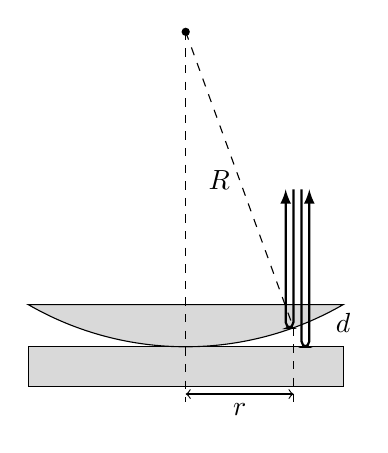
\begin{tikzpicture}
        \filldraw[color=black, fill=gray, fill opacity=0.3] (-120:4) arc (-120:-60:4) --cycle;
        \filldraw[color=black, fill=gray, fill opacity=0.3] (-2,-4) rectangle (2,-4.5);

        \fill (0,0) circle (1.5pt);
        \draw[dashed] (0,0) -- (0,-4.7);
        \draw[dashed] (1.37,-3.76) -- (1.37,-4.7);
        \draw[<->] (0,-4.6) -- node[below] {$r$} (1.37,-4.6);
        \draw[dashed] (0,0) -- node[left] {$R$} (-70:4);
        \node at (2,-3.7) {$d$};

        \draw[thick, -latex, rounded corners=2pt] (1.37,-2) -- (-70:4) -- (1.27,-3.76) -- (1.27,-2);
        \draw[thick, -latex, rounded corners=2pt] (1.47,-2) -- (1.47,-4) -- (1.57,-4) -- (1.57,-2);
    \end{tikzpicture}
    \caption{牛顿环干涉}
\end{figure}

\paragraph{干涉条件}根据图形关系可得两束光线的光程差为$2d$,使用凸透镜半径$R$和干涉点到圆心距离$r$后可表示为$\frac{r^2}{R}$,结合反射相变可得如下干涉条件。
\begin{itembox}[l]{牛顿环干涉条件}
    \begin{equation*}
        2d=\frac{r^2}{R}=
        \begin{cases}
            2m\cdot\frac{\lambda}{2}&\implies
            \textrm{0相变明线/}\pi\textrm{相变暗线}\\
            (2m+1)\cdot\frac{\lambda}{2}&\implies
            \textrm{0相变暗线/}\pi\textrm{相变明线}
        \end{cases}
    \end{equation*}
\end{itembox}
